\documentclass[xcolor={svgnames}]{beamer}
\usetheme{metropolis}           % Use metropolis theme
\usepackage[utf8]{inputenc}
%\usepackage[brazil]{babel}
\usepackage[normalem]{ulem}
\usepackage{float}
\usepackage{caption}
\usepackage{subcaption}
\usepackage{graphicx}

\usepackage[backend = biber]{biblatex}
%\addbibresource{refs.bib}
\metroset{background=light}
\addbibresource{refs.bib}
\usepackage{tikz}
\usepackage{pgfplots}
\def\checkmark{\tikz\fill[scale=0.4](0,.35) -- (.25,0) -- (1,.7) -- (.25,.15) -- cycle;}
\title{Majoritarian principles in critical junctures: an analysis of Brazil's
  2018 presidential election}

\date{}
\author{Marcelo Veloso Maciel}
\institute{University of California, Irvine}
\begin{document}
\maketitle

% ----------------- NOVO SLIDE --------------------------------
\begin{frame}
\frametitle{Context : electoral success of highly divisive candidates}
  \begin{figure}[H] \centering 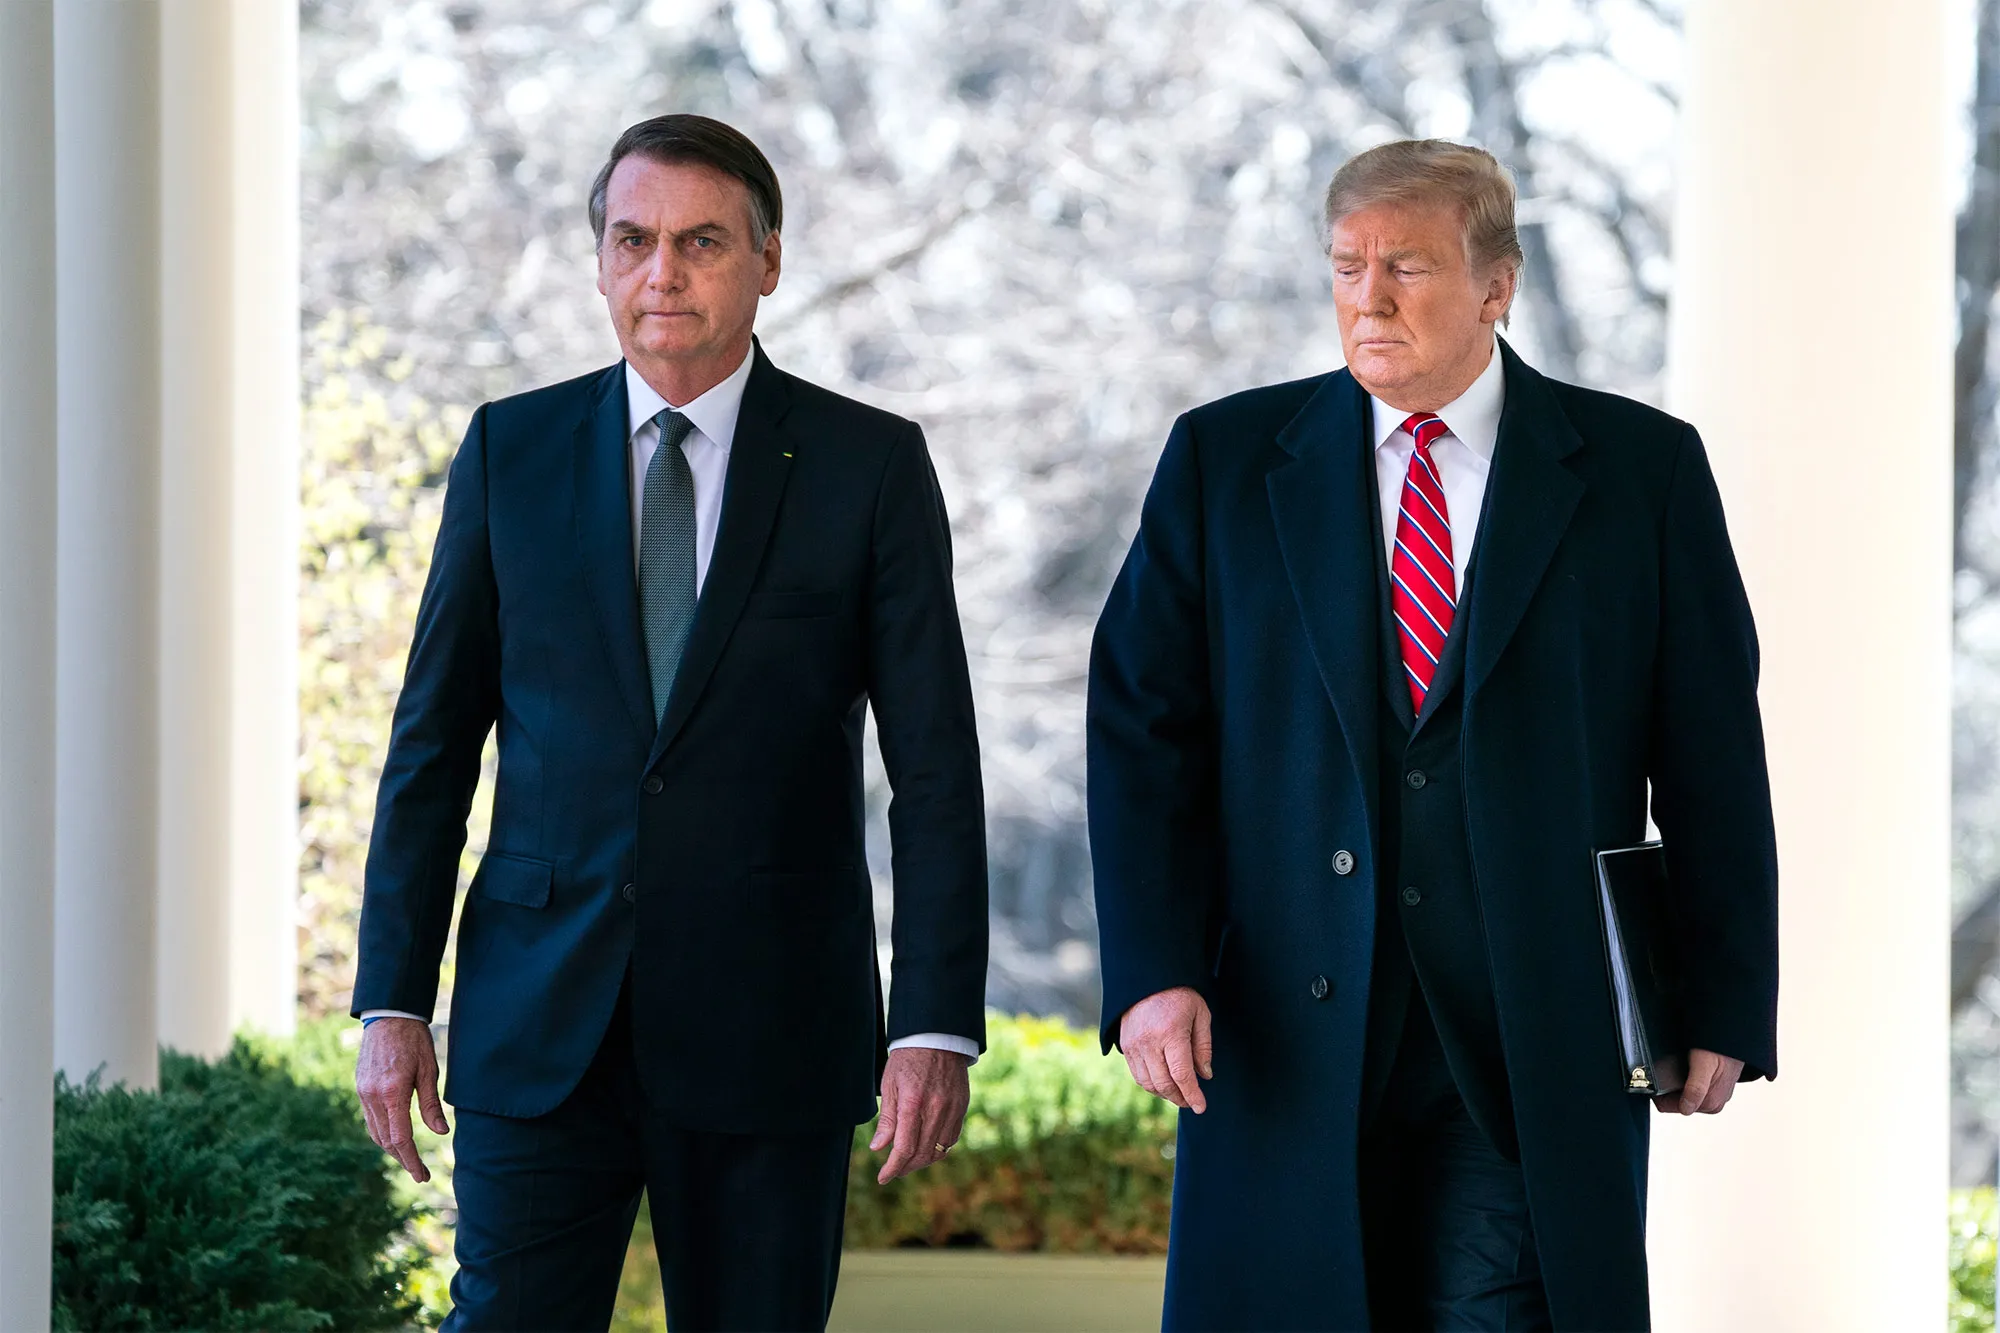
\includegraphics[width=\textwidth]{./trumpolnaro.png}
 %\caption{Jair Messias Bolsonaro and Donald Trump}
 \end{figure}
\end{frame}

\begin{frame}
  \frametitle{Research Question }
  Is the election of divisive or polarizing candidates an artifact of the voting
  methods?
\end{frame}

\begin{frame}
  \frametitle{Prior research}
  \begin{itemize}
    \item \textcite{potthoff2021condorcet} and \textcite{kurrild2018trump} argue
          that Trump might have been a Condorcet loser. \textcite{woon2020trump}
          argue he was in the Core.
    \item \textcite{igersheim22_compar_votin_method} argue that the
          Condorcet,Borda, Utilitarian winner was actually Sanders.
  \end{itemize}
\end{frame}

\begin{frame}
  \frametitle{Hypothesis}
  I expected similar results in the Brazilian 2018 presidential election.
  Particularly, I expected him to have neither ``pairwise'' nor high
  ``positional'' mandate.
\end{frame}
\begin{frame}
  \frametitle{Background on the Election }
  \begin{itemize}
  \item Abstention: 20\%
  \item White/Null: 8.79\%
  \item Others: 7.19\%
  \end{itemize}
\end{frame}

\begin{frame}
  \frametitle{Top four candidates' first round shares }
{\centering
  \begin{tikzpicture}

\begin{axis} [ybar,
  xtick=data,
  height=7cm,width=12cm,
      symbolic x coords={Haddad,Ciro, Alckmin, Bolsonaro},
      bar shift=0pt,
      point meta=y*100,
             nodes near coords={\pgfmathprintnumber\pgfplotspointmeta\%},
             bar width=20pt,
             ytick style={draw=none },
             ytick = \empty,xtick pos=left,]

\addplot[black] coordinates {
  (Haddad,0.2928) (Ciro,0.1247) (Alckmin,0.0476) (Bolsonaro,0.469)};
\end{axis}

\end{tikzpicture}
}
\end{frame}

\begin{frame}
  \frametitle{Data}

   I use a representative street survey done by DataFolha a week before the first round of the presidential election. A pairwise comparison of the top 4 candidates was the only question I analyzed.

\end{frame}

\begin{frame}{Data Preprocessing}
  \begin{itemize}
    \item Not all respondents compared all candidates. I imputed the data with polytomous regressions\footnote{Using the \textbf{\textsf{R}} package
          \(\operatorname{mice}.\)}.
    \item There was a discrepancy between the survey and the result of the first
          round. I transferred while respecting Kemeny's distance, and picked
          the transferrence with minimal euclidean distance to the result.
  \end{itemize}
\end{frame}
\begin{frame}
  \frametitle{Method - Saari's Geometry of Voting }
  \begin{itemize}
    \item Positional Voting methods are weighting systems: assign points to
          candidates according to their positions in the rankings. Then sum
          those points to get the candidates' scores.
          \begin{itemize}
            \item Plurality: (1,0,0);
            \item Antiplurality: (1,1,0);
            \item Borda: (2,1,0).
          \end{itemize}

     \item They can be normalized:
    \begin{itemize}
      \item Three candidates: \((1,s,0)\) where \(0 \leq s \leq 1\);
      \begin{itemize}
        \item Borda becomes \((1,{1 \over 2},0)\);
      \end{itemize}
      \item Four candidates: \((1,s_{1},s_{2},0)\),
            where \(0 \leq s_{2} \leq s_{1} \leq 1\).
          \end{itemize}
\end{itemize}
  \end{frame}

\begin{frame}
  \frametitle{Method - Saari's Outcome Triangle}
\begin{figure}[H] \centering 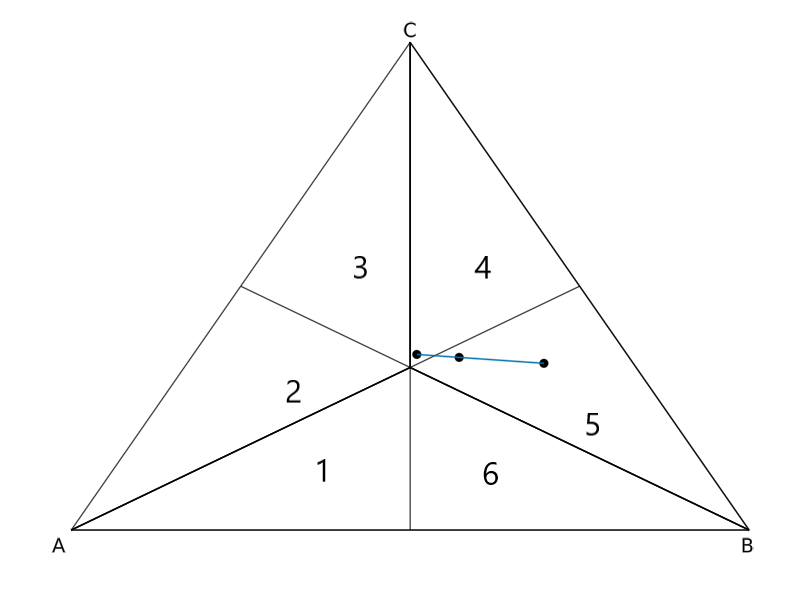
\includegraphics[width=\textwidth]{../images/simpletriangle.png}
 \caption{Saari's outcome simplex}
 \label{fig:saari_nurmi}
\end{figure}
\end{frame}


\begin{frame}
  \frametitle{Frequencies at each position in the ranking}
\begin{figure}[!h] \centering

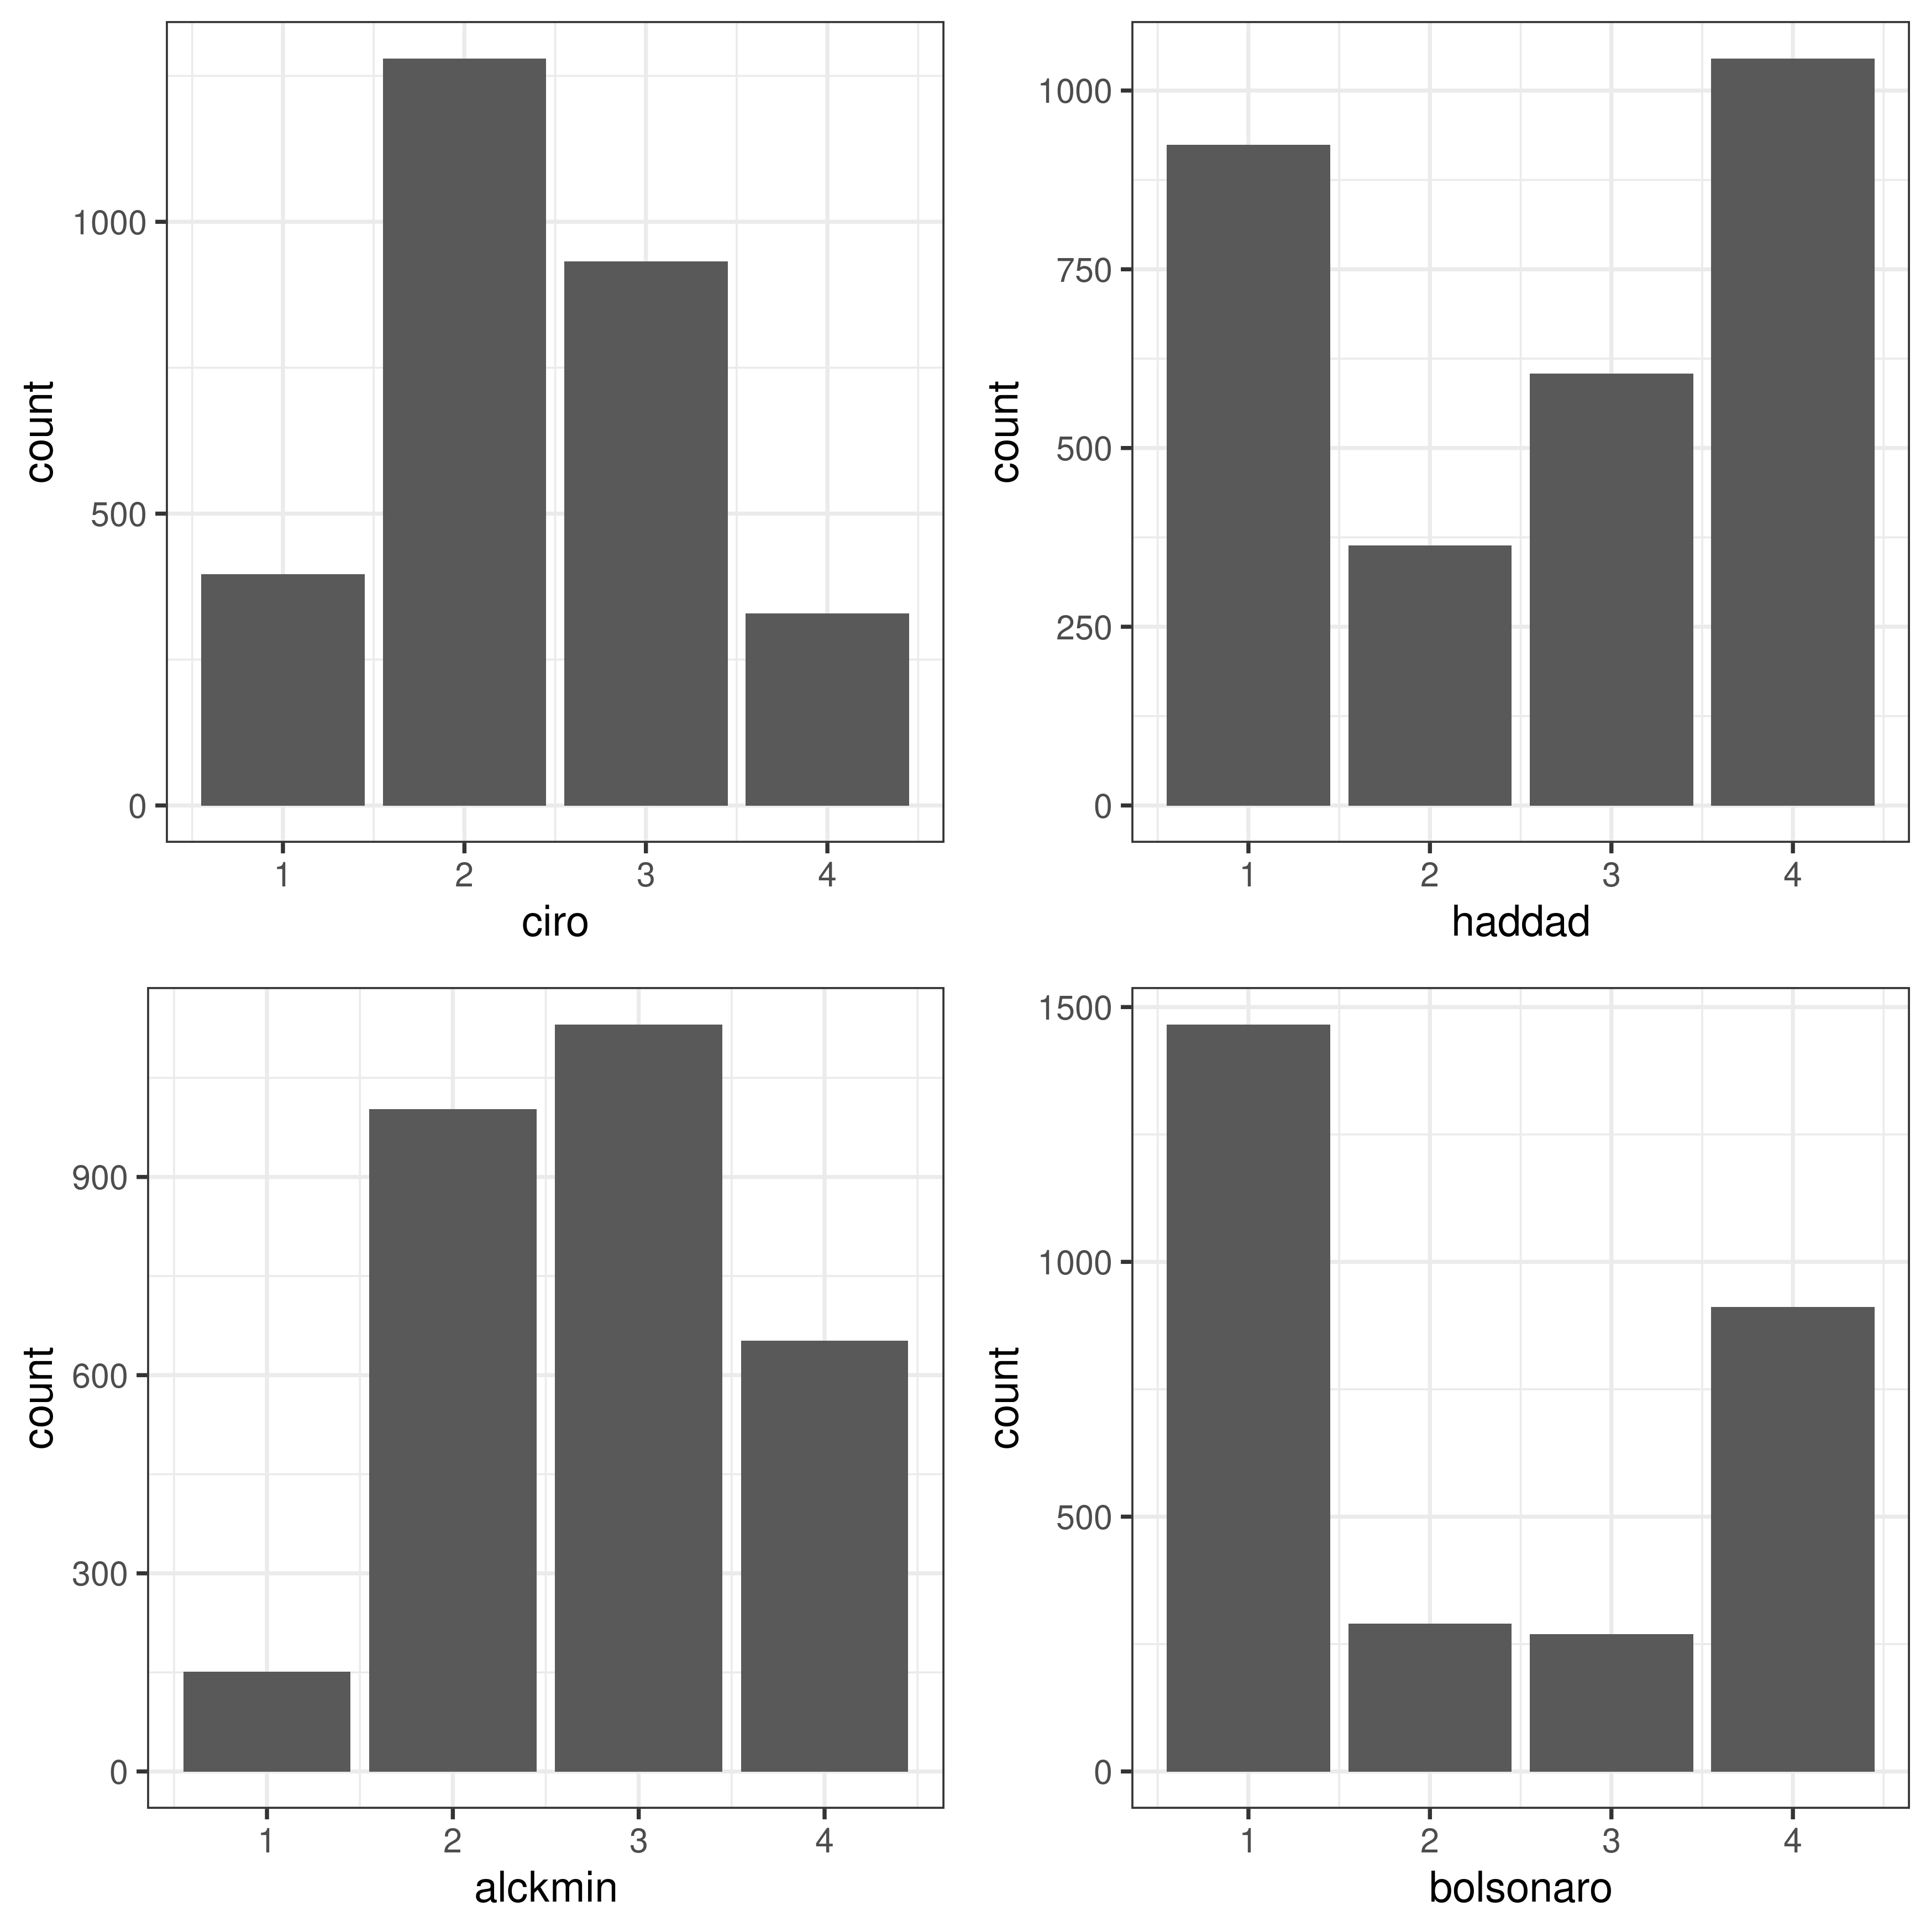
\includegraphics[width=0.85\textwidth, height = 0.85\textheight]{../images/corrected1_indexes_plot.png}



\end{figure}
\end{frame}

\begin{frame}
  \frametitle{ Pairwise Majority Comparisons}

\begin{table}[!h]
\centering
\begin{tabular}{rrrrr} & Alckmin & Bolsonaro & Ciro & Haddad \\\hline Alckmin &
  - & -12.63\% & -16.99\% & 8.27\% \\ Bolsonaro & \textcolor{green}{12.63\%} & -
  & \textcolor{green}{5.48\%} & \textcolor{green}{7.46\%} \\ Ciro & 16.99\% &
  -5.48\% & - & 16.65\% \\ Haddad & \textcolor{red}{-8.27\%} &
  \textcolor{red}{-7.46\%} & \textcolor{red}{-16.65\%} & - \\\hline

\end{tabular}
\end{table}

\end{frame}

\begin{frame}
  \frametitle{Borda Count outcome }

\begin{table}[!h]
\centering
          \begin{tabular}{rrr} \hline & Borda Score & Standardized Borda Score\\
            \hline
            Alckmin & 7029 & 0.464 \\ Bolsonaro & 7718 & \textbf{0.543} \\ Ciro & \textcolor{green}{7756} & \textbf{0.547}\\
            Haddad & 6867 & 0.446 \\ \hline
\end{tabular}
\end{table}
\end{frame}

\begin{frame}
  \frametitle{9 possible positional outcomes}
\begin{figure}[!h] \centering 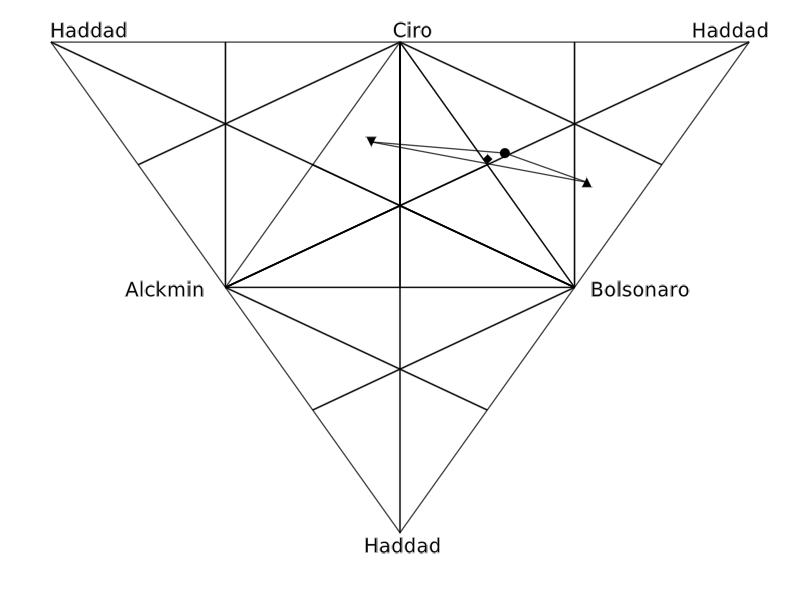
\includegraphics[width=\textwidth]{../images/opened_tetrahedron1.png}
 %\caption{Saari's opened tetrahedron }
 
\end{figure}

\end{frame}

\begin{frame}
  \frametitle{Counterfactual Positional Victories }
\begin{table}[H]
  \centering
  \begin{tabular}{rrrrr}
    \hline
     & Alckmin & Bolsonaro & Ciro & Haddad \\
    \hline
    Alckmin & 0.0 & 0.31 & 0.0 & 0.58 \\
    Bolsonaro & 0.69 & 0.0 & 0.47 & 1.0 \\
    Ciro & 1.0 & 0.53 & 0.0 & 0.81 \\
    Haddad & 0.42 & 0.0 & 0.19 & 0.0 \\\hline\hline
  \end{tabular}
  % \caption{Proportion of victories in the positional voting procedure set}
  \label{tbl:ctn}
\end{table}

\end{frame}

\begin{frame}
  \frametitle{Victory in terms of weights given to the second  (\(s_1\)) and third ( \(s_2\)) positions in the rankings}
\begin{figure}[!h] \centering 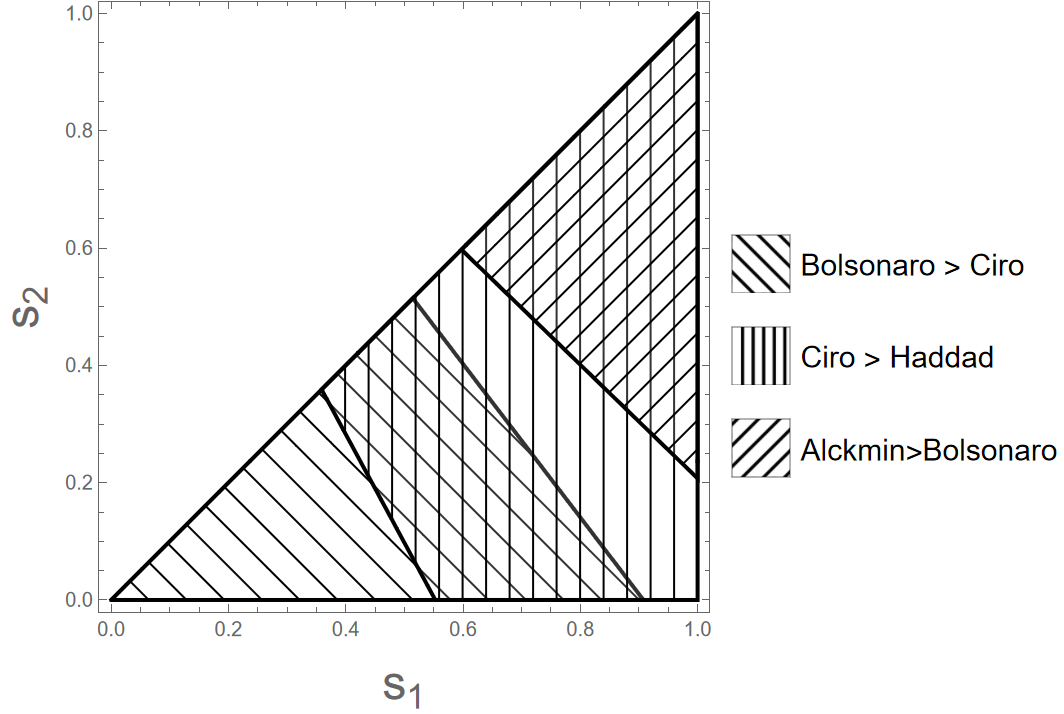
\includegraphics[width=\columnwidth]{../images/counterfactual_triangle.png}
\end{figure}


\end{frame}

% \begin{frame}
%   \frametitle{Alternative Set Stability }

%    \begin{figure}[!h] \centering
%         \begin{subfigure}[b]{0.45\textwidth} \centering
% 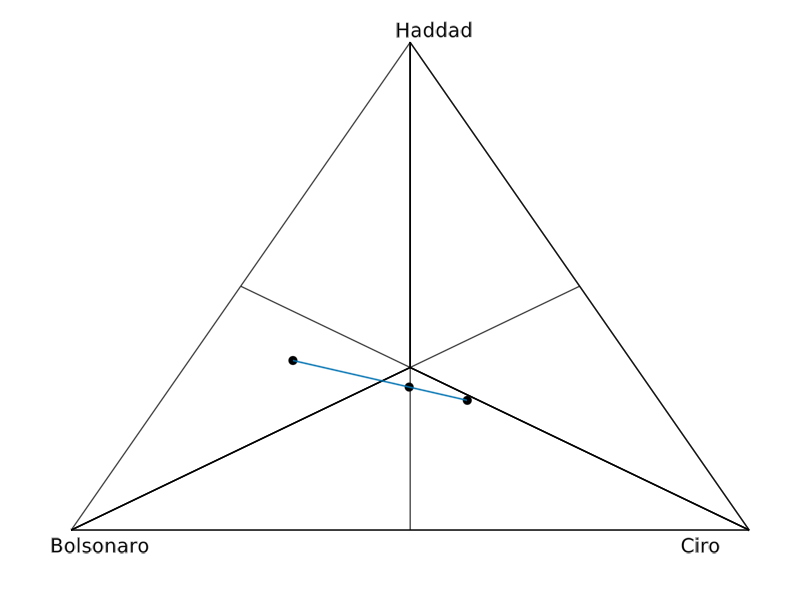
\includegraphics[width=\textwidth]{../images/cw1_nota.png}

%         \end{subfigure} \hfill
%         \begin{subfigure}[b]{0.45\textwidth} \centering
% 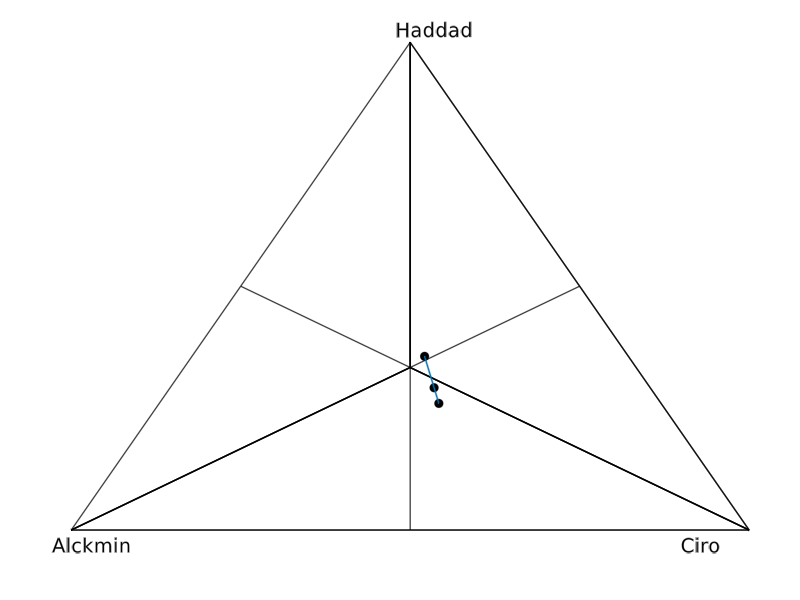
\includegraphics[width=\textwidth]{../images/cw1_notb.png}

%         \end{subfigure} \vskip\baselineskip
%         \begin{subfigure}[b]{0.45\textwidth} \centering
% 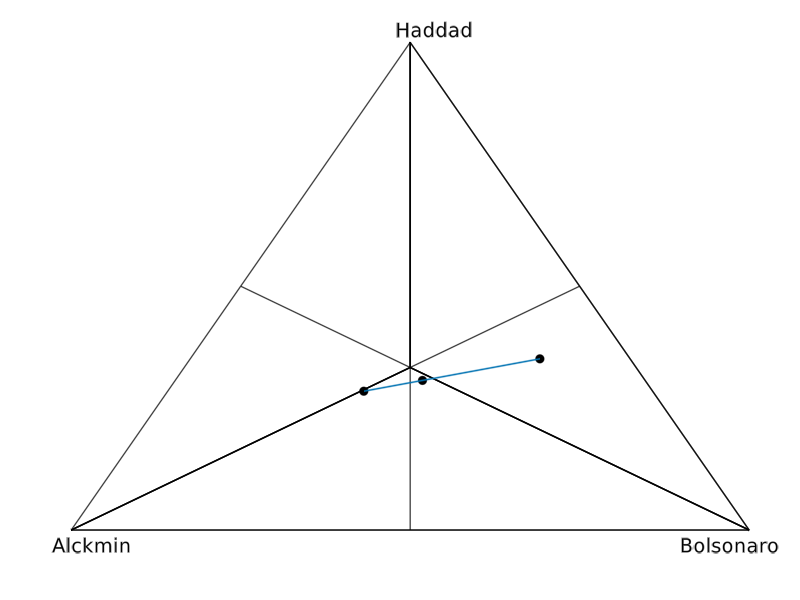
\includegraphics[width=\textwidth]{../images/cw1_notc.png}

%         \end{subfigure} \hfill
%         \begin{subfigure}[b]{0.45\textwidth} \centering
% 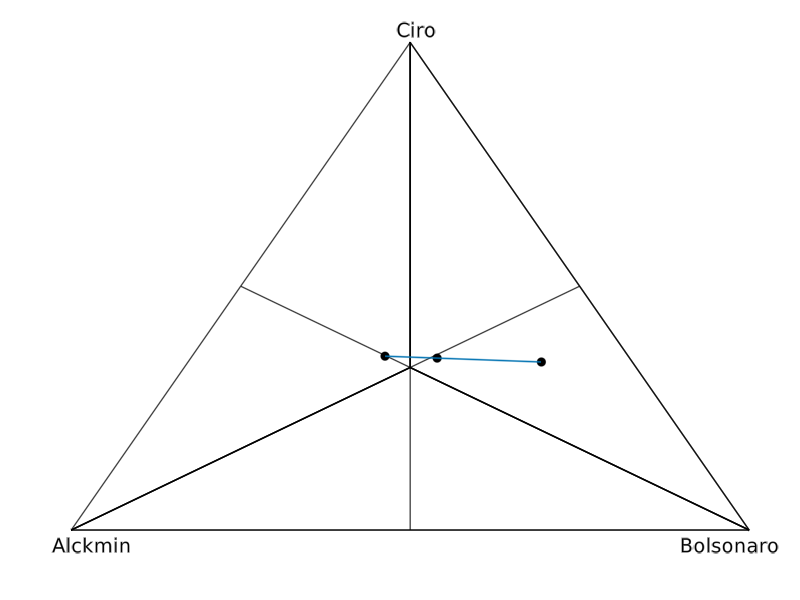
\includegraphics[width=\textwidth]{../images/cw1_noth.png}
%         \end{subfigure}
%         \caption[ Positional results when dropping one candidate ] {\small
% Positional results after dropping one candidate }
%         \label{fig:c1dropping}
%     \end{figure}

% \end{frame}

\begin{frame}
  \frametitle{Discussion}
  \begin{itemize}
    \item We can't conclude Bolsonaro's victory was an institutional fluke.
          However, there is a conflict between the visions of Condorcet and
          Borda in this case:
              \begin{itemize}
      \item pairwise mandate: \textcolor{green}{\checkmark}
      \item positional mandate: \textcolor{red}{\(\times\)}
    \end{itemize}
  \end{itemize}
  \begin{minipage}{.45\linewidth}
  \begin{itemize}
    \item They perfectly match had he not run.
  \end{itemize}
\end{minipage}
\begin{minipage}{.45\linewidth}
\centering
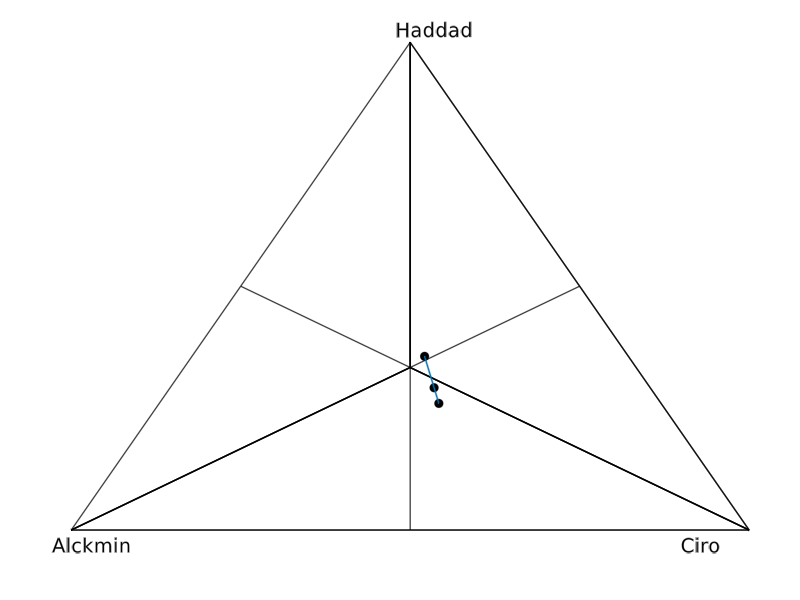
\includegraphics[width=\linewidth]{../images/cw1_notb.png}

\end{minipage}

\end{frame}

\begin{frame}
  \frametitle{Limitation and next steps}
   \begin{itemize}
     \item  Use other variables in the dataset, particularly in the imputation.
     \item   Such counterfactual analysis can be done for any dataset we can recover the (partial) rankings.
      \item \(\bigstar\) Why did the CW and BW diverge? Size of the Condorcet Component \parencite{saari2000mathematicaloriginal}?
    \end{itemize}
\end{frame}

\frame[allowframebreaks]{

\tiny\printbibliography
}

  \end{document}


%% \section*{Referências}
%% \begin{frame}[allowframebreaks]{Referências}
%% \printbibliography[heading=none]
%% \end{frame}


%%% Local Variables:
%%% mode: latex
%%% TeX-master: ""
%%% End:
